% IntelliERP / TRACE journal article, IEEE journal format (IEEEtran).
% Compile on Overleaf (IEEEtran is built in) or locally with: pdflatex, bibtex, pdflatex, pdflatex.
\documentclass[journal]{IEEEtran}
\usepackage[T1]{fontenc}
\usepackage{cite}
\usepackage{amsmath,amssymb}
\usepackage{booktabs,array}
\usepackage{xcolor}
\usepackage{tikz}
\usetikzlibrary{arrows.meta,positioning}
\usepackage[hidelinks]{hyperref}
\newcommand{\pending}[1]{\textcolor{red}{[#1]}}
% Run-in italic paragraph headings (IEEEtran would letter them as a), b), ...).
\renewcommand{\paragraph}[1]{\par\textit{#1}\enspace}
% Results still running (Gemma judge; MiniCheck on natural answers); replaced when complete.
\newcommand{\HELDOUTBASELINES}{LLM judge (gemma-4-31b-it) & 76/102 (75\%; 65--82) & 38/50 & 38/52 & 7/103 (7\%; 3--13) \\
MiniCheck & 38/102 (37\%; 28--47) & 20/50 & 18/52 & 22/103 (21\%; 15--30) \\}
\newcommand{\HELDOUTMINIGEMMA}{\paragraph{Comparison with MiniCheck.} MiniCheck detected 38 of the 102 errors (37\%), significantly fewer than
TRACE-hybrid (46 errors detected only by TRACE-hybrid, 14 only by MiniCheck; Holm-adjusted $p<0.001$), and
raised false alarms on 22 of 103 paraphrases (21\%). It was best on rule values (9 of 14) and weakest on
derived results (4 of 15) and permissions (2 of 9). MiniCheck asks whether the evidence \emph{entails} a
sentence, not whether it contradicts it, so every sentence the evidence does not state in so many words is
flagged: it flagged at least one sentence in 45 of the 52 original texts. Its false alarms on paraphrases were
correct sentences of three kinds: a company rule in other words (``company policy classifies zero stock with
ongoing sales as a Critical stockout hazard''), a sentence combining several figures, and the assistant's own
actions (``a draft purchase order has been generated'', ``I am unable to approve or submit this order''). A
checker trained on general-domain entailment cannot tell a reworded rule from a wrong one; the typed
assertions and the rule keys of TRACE make that comparison explicit.}
\newcommand{\NATURALBASELINES}{LLM judge (Gemma)$^{*}$ & 11/14 (79\%; 52--92) & 25/145 (17\%; 12--24) \\
MiniCheck & 14/19 (74\%; 51--88) & 41/503 (8\%; 6--11) \\}
\newcommand{\FPQGEMMA}{gemma-4-31b-it & off & 41/44 (93\%; 82--98) & 16/19 & 12/12 & 13/13 & -- \\
 & patterns & 41/44 (93\%; 82--98) & 16/19 & 12/12 & 13/13 & 4 \\
 & TRACE & 41/44 (93\%; 82--98) & 16/19 & 12/12 & 13/13 & 8 \\}
\newcommand{\GEMMASCOPE}{could not judge 8 of those answers, for which its API returned a server error on every attempt}
\newcommand{\attr}[1]{\texttt{#1}}

\begin{document}

\title{IntelliERP: Evidence-Grounded Hallucination Detection and Verification for LLM-Based ERP Decision
Support}
\author{Mohammad Yasin Siddique, Zeyad Ahmed, and Ashish K. Soni%
\thanks{M. Y. Siddique is with the Department of Computer Science and Engineering, G H Raisoni College of
Engineering, Nagpur, India, and carried out this work as a mobility research intern at the Faculty of Data Science
and Information Technology, INTI International University, Nilai, Malaysia (e-mail: my.siddique2005@gmail.com).}%
\thanks{Z. Ahmed is with the Faculty of Data Science and Information Technology, INTI International University,
Nilai, Malaysia.}%
\thanks{A. K. Soni is with the Department of Computer Science and Engineering, G H Raisoni College of Engineering,
Nagpur, India.}}
\markboth{}{Siddique \MakeLowercase{\textit{et al.}}: Evidence-Grounded Hallucination Detection and Verification for LLM-Based ERP Decision Support}

\maketitle

\begin{abstract}
Large language models (LLMs) are being connected to enterprise resource planning (ERP) systems to answer
questions, explain risks and propose actions. Current ERP agents control what the model may do, but not
whether what it says is true: a grounded assistant can still misstate a stock level, invent a threshold or
claim a permission it lacks. We present TRACE (Typed Run-time Assertion Checking for Enterprise assistants),
built into IntelliERP, a decision-support system for sales, inventory and procurement. TRACE turns each
factual statement of an answer into a typed assertion over the database state, the analytics' results and
the company's rules and permissions (64 attributes), and evaluates it with the system's own code before
the user sees the answer. A language model only extracts assertions; their truth is decided
deterministically, so every error can be attributed to extraction, coverage of the language or a
verification function. On a held-out test generated after TRACE was frozen (102 model-written errors and
103 paraphrases by two writer models), TRACE detected 69\% of the errors with false alarms on 4\% of the
paraphrases, against 15\% for a pattern-based verifier ($p<10^{-15}$) and 37\% with 21\% false alarms for
MiniCheck. Two LLM judges given the same evidence detected 78\% and 75\%, not significantly more; one raised
significantly more false alarms (17\%), the other did not (7\%). No miss and no false alarm came from a
verification function. On the assistant's own answers (300 sampled sentences, 7.3\% of the checkable ones
false), TRACE found only 4 of 19 errors, because most natural errors misstate definitions or relations
between figures that the language does not cover; grounding in a knowledge base lowered the natural error
rate from 26\% to 2.4\%. Verification did not measurably change answers to false-premise questions, and two
of its false alarms made correct answers wrong. The results show where deterministic verification is strong
and what it still needs.
\end{abstract}

\begin{IEEEkeywords}
Enterprise resource planning, large language models, hallucination, run-time verification, decision
support, claim verification.
\end{IEEEkeywords}

% =====================================================================================================
\section{Introduction}

Enterprise software is acquiring conversational assistants. In ERP systems they answer questions such as
``which products will run out first?'' or ``should we reorder this item, and from whom?'', explain the
risks an analytics engine has found, and increasingly act: recent systems let LLM agents execute purchasing
and inventory transactions on a real ERP \cite{liu2026agenticerp, yang2025finrobot}. The research on these
agents has concentrated on what they \emph{do}. Benchmarks score their actions and business outcomes
\cite{zhang2026erpbench, vishwakarma2025enterprisebench, han2026cfo}; safety comes from risk tiers that
route consequential actions to a human \cite{liu2026agenticerp} or from admissibility checks on proposed
actions \cite{misra2026admitbench}. What the assistant \emph{says} is checked, if at all, by another LLM.
The closest system states plainly that its run-time gate is ``not a bound on how often a hallucinated or
mis-calibrated decision is proposed'' and that hallucination frequency was not measured
\cite{liu2026agenticerp}.

Statements matter because people act on them. A buyer who is told that a product's stock is above its
reorder point does not reorder; a manager who is told that procurement managers cannot approve orders
escalates unnecessarily. Explanations can make people accept AI advice whether it is right or wrong
\cite{bansal2021whole}, while signals that make checking cheap reduce over-reliance
\cite{vasconcelos2023overreliance}. Grounding the model in tool results and documentation reduces errors
but does not remove them: in our own system, a grounded assistant that answered all 86 evaluation questions
correctly on keyword scoring still produced false qualitative statements that the scoring missed (Section
\ref{sec:v1}).

Checking claims against data is an old idea. Database research has long verified claims in published
documents by translating them into SQL \cite{jo2019aggchecker, karagiannis2020scrutinizer}, and recent
systems let LLMs write the queries \cite{jayasekara2025cedar, theologitis2025thucy}. Hallucination
detectors judge text against reference documents \cite{tang2024minicheck, niu2024ragtruth}, against the web
\cite{wei2024longform}, or against the model's own samples \cite{manakul2023selfcheckgpt,
farquhar2024semantic}. None of these checks an assistant's statements \emph{inside} the enterprise system,
\emph{before} they are shown, against the system's own business semantics: stock and orders, but also risk
levels, reorder rules, what-if simulations, company thresholds and role permissions.

We take the view of run-time assertion checking from software engineering
\cite{meyer1992contract, clarke2006rac}: each factual sentence of an answer is an assertion about the
state of the business, and it can be checked by code. The contributions are:
\begin{enumerate}
\item \textbf{A typed assertion language for enterprise assistants} with three families and sources of
truth: state (the database), derived (the analytics) and policy (executable rules and the permission map),
covering 64 attributes, 24 rule keys and 21 actions (Section \ref{sec:language}).
\item \textbf{TRACE}, a verifier in which an LLM only extracts assertions into a validated schema and
deterministic functions decide them; with a conditional soundness property and an error decomposition
that attributes every miss and false alarm (Sections \ref{sec:problem}, \ref{sec:trace}).
\item \textbf{An evaluation protocol} for statement verification in an enterprise assistant: development
and held-out sets of model-written errors with two writers and stratified error types, rules fixed before
the test, attributed detection, natural errors found by pooling, and false-premise
questions to measure the end-to-end effect (Section \ref{sec:evaluation}).
\item \textbf{An empirical comparison} with a pattern-based verifier, an LLM judge given the same evidence
and a trained small fact-checker, including cost and repeatability (Section \ref{sec:results}).
\end{enumerate}

% =====================================================================================================
\section{Related work}
\label{sec:related}

\paragraph{LLM agents in ERP.} Agentic ERP \cite{liu2026agenticerp} runs a planner--executor--reflector
graph over Odoo and gates actions by risk tier; FinRobot \cite{yang2025finrobot} builds finance workflows
with inserted risk controls; ERPBench \cite{zhang2026erpbench}, EnterpriseBench
\cite{vishwakarma2025enterprisebench} and EnterpriseArena \cite{han2026cfo} evaluate agents on tasks and
outcomes. Contract2Plan \cite{agarwal2026contract2plan} extracts a typed constraint schema from contracts
and puts a solver-based gate before a plan is emitted, the closest method to ours, but for optimisation
inputs rather than an assistant's statements. ADMITBench \cite{misra2026admitbench} judges the admissibility
of proposed actions of industrial advisories against a plant profile. Freeman et al.\
\cite{freeman2026epistemic} reduce industrial hallucination by prompting and measure it with an LLM judge.
Earlier work connects LLMs to enterprise data through SQL \cite{ruizgomez2025erp, sequeda2023kg,
lei2025spider2, li2023bird} or optimisation models \cite{li2023optiguide}; none verifies the resulting
statements.

\paragraph{Verifying claims against structured data.} AggChecker \cite{jo2019aggchecker} and Scrutinizer
\cite{karagiannis2020scrutinizer} translate claims in documents into SQL; CEDAR
\cite{jayasekara2025cedar} and Thucy \cite{theologitis2025thucy} use LLMs to write the queries; TabFact
\cite{chen2020tabfact} and QuanTemp \cite{venktesh2024quantemp} are benchmarks for table and numerical
claims; ProgramFC \cite{pan2023programfc} decomposes claims into programs. These systems work offline on
documents and depend on generated queries; business rules, permissions and simulations are outside
relational algebra.

\paragraph{Hallucination detection.} Self-consistency \cite{manakul2023selfcheckgpt} and semantic entropy
\cite{farquhar2024semantic} detect confabulation without external data but miss consistent mistakes. SAFE
\cite{wei2024longform} decomposes answers into facts and checks them by search; MiniCheck
\cite{tang2024minicheck} is a small trained checker against grounding documents; RAGTruth
\cite{niu2024ragtruth} annotates natural errors in retrieval-augmented answers; Claimify
\cite{metropolitansky2025claimify} studies claim extraction; CRITIC \cite{gou2024critic} lets the model
correct itself with tools. In all of them, a model decides whether a statement is true. LLM judges have
known problems of consistency and bias \cite{gu2024judge}.

\paragraph{Run-time enforcement.} AgentSpec \cite{wang2026agentspec} and ProbGuard \cite{wang2026probguard}
enforce rules on agent \emph{actions} at run time. TRACE applies the same idea to \emph{statements}.

% =====================================================================================================
\section{Problem formulation}
\label{sec:problem}

\paragraph{System of record.} Let $S=(D,R,F)$ be the system of record: the database state $D$, the rule
registry $R$ (code constants, status and risk rules, the permission map) and deterministic analytics $F$
(risk assessment, reorder rule, forecasts, what-if simulation, rankings), all implemented as tested code.

\paragraph{Assertions.} An assertion is a tuple
$a=(q, s, \alpha, \theta, v, \tau, \pi)$: the quoted words $q$ of the text it comes from, a subject $s$
(a product, supplier, purchase order, role, rule key, risk level or stock status), an attribute $\alpha$
from a fixed catalogue, a comparator $\theta\in\{=,\neq,<,\le,>,\ge\}$, a value $v$ (a number, date,
category, entity, truth value, action, or a reference $@\beta$ to another attribute of the same subject or
$@s'$ to the same attribute of another subject), a tense $\tau\in\{\text{present},\text{past}\}$ and scenario
parameters $\pi$ (demand change, delay, order quantity, horizon, period). Each attribute has a family
$\phi(\alpha)\in\{\text{state},\text{derived},\text{policy}\}$, a value kind and a function
$\mathrm{val}_\alpha(s,\pi;S)$ that returns its true value or fails.

\paragraph{Verdicts.} An assertion is \emph{decidable} in $S$ if its subject $s$ can be resolved,
$\mathrm{val}_\alpha$ returns a value, $v$ is well-typed for $\alpha$, and, when $\tau$ is past, $\alpha$ is
a recorded fact. The verdict is
\[
V(a,S)=\begin{cases}
\text{unverifiable} & \text{if } a \text{ is not decidable in } S,\\
\text{supported} & \text{if } \mathrm{val}_\alpha(s,\pi;S)\ \theta\ v,\\
\text{contradicted} & \text{otherwise.}
\end{cases}
\]
$V$ is computed from $S$ alone. A subject written as a well-formed identifier that does not exist makes the
assertion contradicted, since the statement presupposes something false.

\paragraph{Extraction and faithfulness.} An extractor $E$ maps a text $t$ to a set of assertions. An
assertion is \emph{faithful} to its sentence if a careful reader would agree that the sentence asserts
exactly $a$: same subject, attribute, direction and value, in the same scenario and tense.

\paragraph{Conditional soundness.} If $a$ is faithful and $\mathrm{val}_\alpha$ is correct, then
$V(a,S)=\text{supported}$ only if the sentence is true with respect to $S$, and
$V(a,S)=\text{contradicted}$ only if it is false. This follows from the definition: the comparison is
evaluated on the true value. The guarantee is conditional, and its value is that it localises error: a
wrong verdict can only come from (i) an unfaithful extraction, (ii) a sentence the language cannot express,
or (iii) a defect in a verification function, and each can be measured separately (Section
\ref{sec:results}). An LLM judge offers no such decomposition.

% =====================================================================================================
\section{IntelliERP}
\label{sec:v1}

IntelliERP is a decision-support system for sales, inventory and procurement with a React front end, a
FastAPI back end and PostgreSQL, on a wholesale dataset derived from Microsoft's Wide World Importers (227
products, 72,696 sales lines) with simulated stock, suppliers and purchase orders. Deterministic analytics
compute demand and its trend, days of cover, observed lead times, a four-level stockout risk, an
order-up-to reorder quantity, forecasts chosen by backtest error, supplier on-time rates and delay trends,
and day-by-day what-if projections. The assistant answers by calling 15 permission-checked tools that wrap
the same services as the web pages, and is grounded in a 41-passage knowledge base whose thresholds are
generated from the code constants. Its only action is a draft purchase order, which passes the same
validation as any order and must be submitted and approved by people, the approver being different from
the creator.

The first version verified answers in two ways: every number had to be traceable to a tool result or
passage, and twelve kinds of qualitative claim (below safety stock, demand rising, delivery in time, risk
levels and others) were recognised by patterns and checked against the product's facts. On 86 questions in
repeated runs the grounded assistant passed 84--86 of 86, and an open-weight model passed 86 of 86. The
claim verifier, frozen before testing, detected 77\% of model-written errors \emph{within its twelve claim
kinds} on unseen text with 2\% false alarms; over \emph{all} injected errors it detected only 36--42\%. The
errors it could not express were about permissions, existence, scenario premises, comparisons between
products, supplier relations, validation rules and forecast methods. TRACE was designed to cover them.

% =====================================================================================================
\section{The assertion language}
\label{sec:language}

Table~\ref{tab:families} summarises the language. The catalogue is a single list in code from which both
the extraction prompt and the verifier are generated, so the two cannot drift apart.

\begin{table*}[t]
\centering\small
\caption{Assertion families, sources of truth and examples (64 attributes).}
\label{tab:families}
\begin{tabular}{@{}p{1.8cm}p{4.3cm}p{11.0cm}@{}}
\toprule
Family & Source of truth & Attributes (examples) \\
\midrule
State (31) & database, through the services used by the tools & stock on hand, safety stock, reorder level,
stock status, warehouses, units on order, overdue units, units awaiting approval, next delivery date,
primary supplier, supplied by, price, units sold and revenue over a period; supplier status and products
supplied; purchase-order existence, status, quantity, product, supplier, expected and actual delivery;
counts by stock status \\
Derived (30) & analytics engine & average daily demand, demand trend, days of cover, projected stockout
date, lead time, inventory position, reorder point, suggested quantity and supplier, stockout risk level,
forecast method and weekly forecast, what-if unmet demand, stockout date, ending stock and days below
safety stock, revenue and units-sold rank; supplier on-time rate, delays, lead time, delivery risk level
and delay trend; counts by risk level \\
Policy (3) & code constants and permission map & \attr{policy\_value} over 24 rule keys (e.g.\ the
rising-demand threshold, the review period, supplier risk thresholds, the maximum order quantity);
\attr{role\_can} and \attr{assistant\_can} over 21 actions, with separation of duties \\
\bottomrule
\end{tabular}
\end{table*}

Table~\ref{tab:examples} shows statements from the three families as the verifier judges them on the
system's data.

\begin{table*}[t]
\centering\footnotesize
\caption{Statements, their assertions and TRACE's verdicts on the system's data (output of the verifier).}
\label{tab:examples}
\begin{tabular}{@{}>{\raggedright\arraybackslash}p{5.4cm}>{\raggedright\arraybackslash}p{5.8cm}p{1.8cm}>{\raggedright\arraybackslash}p{3.6cm}@{}}
\toprule
Statement & Assertion & Verdict & What the data says \\
\midrule
``71 units on hand, above the reorder point of 112'' & \attr{stock\_on\_hand}(P004) $>$ \attr{@reorder\_point} &
contradicted & 71 on hand, reorder point 112 \\
``24 open orders, 9 of them overdue'' & \attr{overdue\_orders}(S010) $=$ 9 & contradicted & 7 \\
``demand counts as rising sharply at 25\% or more'' & \attr{policy\_value}(rising\_\allowbreak sharply\_\allowbreak pct) $=$ 25 &
contradicted & 15 \\
``a procurement manager cannot approve purchase orders'' & \attr{role\_can}(procurement manager) $\neq$
approve & contradicted & allowed \\
``I can approve purchase orders for you'' & \attr{assistant\_can} $=$ approve & contradicted & not allowed \\
``if demand rises 25\%, 328.4 units would go unmet over 60 days'' & \attr{scenario\_unmet\_demand}(P062;
$+$25\%, 60 days) $=$ 328.4 & supported & 328.4 (simulation re-run) \\
``P184 will run out before P155'' & \attr{days\_of\_cover}(P184) $<$ \attr{@P155} & supported & 1.6 against
39 days \\
``Product P999 is out of stock'' & \attr{stock\_on\_hand}(P999) $=$ 0 & contradicted & no product P999 \\
\bottomrule
\end{tabular}
\end{table*}

\paragraph{Design choices.}
\begin{itemize}
\item \emph{Comparisons are first-class.} ``Stock is below safety stock'' is
\attr{stock\_on\_hand} $<$ \attr{@safety\_stock}; ``P184 will run out first'' is
\attr{days\_of\_cover} $<$ \attr{@P167}; ``a product's cover is below its supplier's lead time'' reads the
supplier attribute through the product's primary supplier.
\item \emph{Scenarios are parameters.} A what-if statement is checked by re-running the simulation with the
stated parameters; the baseline is the scenario with no change.
\item \emph{Policy values are read from code.} Rule values are the constants the analytics use, and
permissions come from the same map that the API enforces, so the verifier cannot disagree with the system
about its own rules. The extraction prompt lists the rule keys but never their values, so an extractor
cannot silently correct a wrong threshold.
\item \emph{Visibility.} An assertion about data the user's role may not see is unverifiable and its true
value is not disclosed.
\item \emph{Time.} Present-state attributes are not judged in the past tense (``it ran out last week'');
recorded facts such as an order's delivery history are.
\end{itemize}

% =====================================================================================================
\section{TRACE}
\label{sec:trace}

\begin{figure*}[t]
\centering
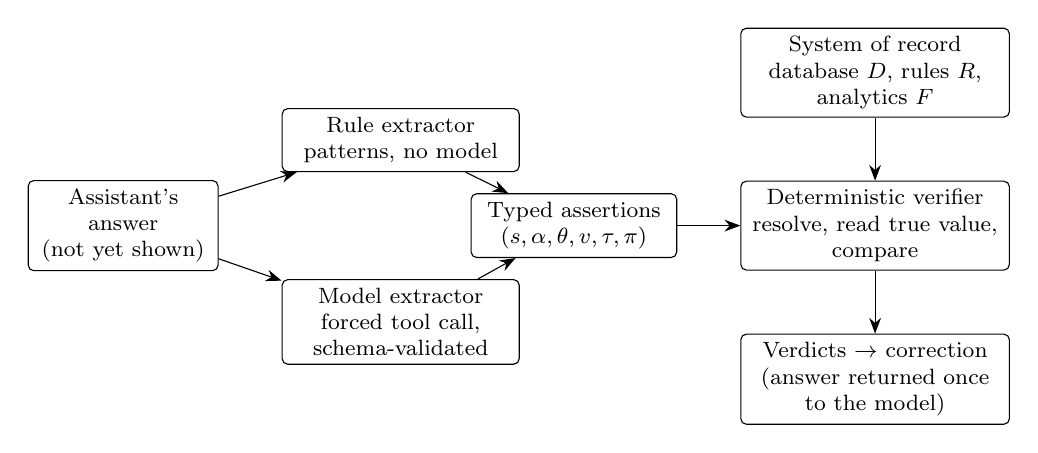
\begin{tikzpicture}[box/.style={draw, rounded corners=2pt, align=center, font=\footnotesize, minimum height=8mm,
  inner sep=3pt}, arr/.style={-{Stealth[length=2mm]}}]
\node[box, text width=2.2cm] (text) {Assistant's answer\\(not yet shown)};
\node[box, text width=2.8cm, above right=1mm and 8mm of text] (rule) {Rule extractor\\patterns, no model};
\node[box, text width=2.8cm, below right=1mm and 8mm of text] (llm) {Model extractor\\forced tool call,\\schema-validated};
\node[box, text width=2.4cm, right=32mm of text] (assert) {Typed assertions\\$(s,\alpha,\theta,v,\tau,\pi)$};
\node[box, text width=3.2cm, right=8mm of assert] (verify) {Deterministic verifier\\resolve, read true value,\\compare};
\node[box, text width=3.2cm, above=8mm of verify] (sor) {System of record\\database $D$, rules $R$,\\analytics $F$};
\node[box, text width=3.2cm, below=8mm of verify] (out) {Verdicts $\rightarrow$ correction\\(answer returned once\\to the model)};
\draw[arr] (text) -- (rule); \draw[arr] (text) -- (llm);
\draw[arr] (rule) -- (assert); \draw[arr] (llm) -- (assert);
\draw[arr] (assert) -- (verify); \draw[arr] (sor) -- (verify); \draw[arr] (verify) -- (out);
\end{tikzpicture}
\caption{TRACE. A language model only extracts assertions; their truth is decided by code that reads the
system of record through the same services as the assistant's tools.}
\label{fig:trace}
\end{figure*}

\paragraph{Extraction.} Figure~\ref{fig:trace} shows the pipeline. Two extractors run. The \emph{model extractor} asks an LLM, through a forced call
of a single tool whose input is the assertion list, to record every checkable statement; the arguments are
validated against the schema and invalid items are dropped and counted. The instructions state that the
comparator must follow the text's words even when the model believes the statement is false. The
\emph{rule extractor} reuses the frozen patterns of the first version (mapped to the language) and adds
patterns for existence, the assistant's capabilities and role permissions; it needs no model call. In
\emph{hybrid} mode both run and a statement contradicted by either is reported.

\paragraph{Verification.} For each assertion: resolve the subject (identifier or exact name), read the true
value through the system's services, parse the asserted value according to the attribute's kind (numbers
equal within rounding to whole numbers or one decimal, or within 0.5\%), and compare. Four safeguards keep
extraction errors from becoming false verdicts:
\begin{enumerate}
\item \emph{Grounding}: an assertion about a product, supplier or order that neither the text, the question
nor the subject of the text names is not judged; the extractor supplied the subject, not the writer.
\item \emph{Ambiguous terms}: some words fit several attributes (``the reorder threshold'' may be the
safety stock, reorder level or reorder point; ``a critical stockout'' the stock status or the risk level;
``pending units'' units on order or awaiting approval). When the quote uses none of the attribute's own
words, the assertion is supported if it holds for any member of the group.
\item \emph{Type checks}: a date compared with a number (in either direction, as in ``October~7'' recorded as
a quantity), a count of orders whose quote gives the figure in units (``73 units pending'' recorded as open
orders), a warehouse said to hold zero units recorded as holding the product, and a strict comparison with
exactly the true figure (typically ``falling ($-$50.6\%)'' read as ``less than $-$50.6'') are not judged.
Names are compared ignoring case and generic words (``Main'' and ``main warehouse'').
\item \emph{Records newer than the data}: a missing purchase order numbered after every recorded order may
have been drafted in the conversation, and is unverifiable rather than contradicted.
\end{enumerate}

\paragraph{Correction.} As in the first version, a chat answer with contradicted statements is returned
once to the model with each statement and the true value; a recommendation must be re-recorded; an insight
is not stored until corrected; a draft purchase order is flagged for its reviewers. Remaining
contradictions are shown to the user.

\paragraph{Implementation.} TRACE is about 1,600 lines of Python in the IntelliERP back end, with 38 unit
test cases in which every expected value is read from the same services rather than copied, and an
integration into the assistant selectable by configuration (patterns, TRACE-rule, TRACE or off).

% =====================================================================================================
\section{Evaluation design}
\label{sec:evaluation}

\paragraph{Research questions.}
RQ1: How well does TRACE detect false statements compared with the pattern-based verifier, an LLM judge and
MiniCheck? RQ2: Which errors remain undetected, and why? RQ3: Does verification with correction change what
the user finally sees? RQ4: What does verification cost, and how repeatable is it?

\paragraph{Development sets.} The three test sets of the first version (59, 60 and 64 model-written single
errors with one paraphrase per text) served as development data for TRACE, because its design was drawn
from what the first version missed on them. Paraphrases that changed the meaning were identified when a
method flagged them, checked by hand and excluded from every method's count (two cases).

\paragraph{Held-out test.} 52 texts that were never read during development: 43 answers of the open-weight
model's run and 9 insights from scans after the development scans. For each text, two writers (Gemini and
Gemma) each produce one rewrite with exactly one statement made false and one paraphrase. Error types are
stratified: each text is assigned in turn one of qualitative, figure, existence, permission, rule and
derived, used when the text allows it. TRACE's source files were frozen by hash before the rewrites were
generated, and the scoring script refuses to run if they have changed.

\paragraph{Scoring rules (fixed before the test).} An injection is valid if the reported old words occur in
the original and the new words in the rewrite. A method \emph{detects} it if it reports more contradicted
statements inside the sentence holding the change than inside the corresponding sentence of the original;
the changed sentence is located by aligning the two texts. A \emph{false alarm} is a paraphrase with more
contradicted statements than its original. Rates have Wilson 95\% intervals \cite{wilson1927}; paired
comparisons use McNemar's exact test \cite{mcnemar1947} with Holm's correction \cite{holm1979}.

\paragraph{Baselines.}
\begin{itemize}
\item \emph{Patterns}: the frozen first-version verifier.
\item \emph{LLM judge}: the model receives the facts of every product and supplier the text names (as the
assistant's tools return them) and the knowledge base's rule, workflow, access and definition passages,
and lists every contradicted statement; temperature 0; Gemini and Gemma; repeated runs on a subset to
measure stability.
\item \emph{MiniCheck} \cite{tang2024minicheck}: the Flan-T5-Large checker run locally, with the same
evidence written as plain sentences; a sentence is flagged when its support is below 0.5.
\end{itemize}

\paragraph{Natural errors.} The random sample is drawn from the 590 stored answers of five runs (430 with
and 160 without the knowledge base). The protocol planned to run every method on all 590 answers. To stay
within the free API quota, the methods were run only on the 211 answers that contain a sampled sentence,
which is all that recall on the sample requires. Precision therefore covers the flags in those 211 answers
only. This deviation was decided before any method had been run on the answers. Every flagged sentence and the seeded random sample of 300 sentences are
annotated blind (the annotator sees the question, the answer, the tool results and the current facts, not
the methods), giving precision for each method and an estimate of the errors all methods miss. The random
sample was drawn, and labelled, before any method had been run on these answers. Labels follow a written
guide: \emph{false} if anything checkable in the sentence is contradicted, \emph{true} if everything
checkable holds, \emph{no-claim} for advice, offers and lead-ins, and \emph{unsure} when the evidence cannot
decide (for example, a claim about last week). Policy statements are judged against the system's rules and
permission map. 183 of the answers were originals of the development sets and are reported separately.

\paragraph{False-premise questions.} 44 questions generated from the database, each assuming something the
data or rules contradict \cite{hu2023falseqa} (19 state, 12 policy, 13 derived; e.g.\ ``Why is demand for
P082 falling so sharply?'' when it is rising). An answer passes when it states the true fact that rebuts the
premise, scored by the same keyword and number rules as the main evaluation; verification plays no part in
scoring. Each question is asked with the verifier off, with patterns and with TRACE, on two models.

% =====================================================================================================
\section{Results}
\label{sec:results}

\subsection{Development sets}

Table~\ref{tab:dev} shows the four methods on the development sets with the final extraction prompt and
verifier, the configuration that was then frozen. On all errors, TRACE-hybrid detected 126 of 183 (69\%)
against 70 of 183 (38\%) for the patterns, and within the patterns' own claim kinds 78 of 87 (90\%) against
69 (79\%). Most of the gain therefore comes from the error types the patterns cannot express. TRACE-rule,
which needs no model call, already adds nine detections (existence and capability statements). False alarms
rose from 1\% to 7\%; all of them are analysed below.

\begin{table*}[t]
\centering\small
\caption{Development sets (perturbations-v2, test-v3, test-v3b; final extraction prompt, gemini-3.5-flash-lite).
Detection: a contradiction the rewrite introduced. In scope: the first version's twelve claim kinds.}
\label{tab:dev}
\begin{tabular}{@{}lrrr@{}}
\toprule
Method & Detected, all errors & Detected, in scope & False alarms \\
\midrule
Patterns (first version) & 70/183 (38\%; 32--45) & 69/87 (79\%; 70--86) & 2/182 (1\%; 0--4) \\
TRACE-rule & 79/183 (43\%; 36--50) & 69/87 (79\%; 70--86) & 2/182 (1\%; 0--4) \\
TRACE-model & 112/183 (61\%; 54--68) & 66/87 (76\%; 66--84) & 10/182 (5\%; 3--10) \\
TRACE-hybrid & 126/183 (69\%; 62--75) & 78/87 (90\%; 81--94) & 12/182 (7\%; 4--11) \\
\bottomrule
\end{tabular}
\end{table*}

\paragraph{What development changed.} Analysing every false alarm led to the four safeguards of Section
\ref{sec:trace}. Two examples: the extractor attached product P001 to a paraphrase that named its product
only by name, without any identifier (grounding); and ``the 69-unit reorder threshold'', where 69 is the
reorder point, was extracted as the reorder level (ambiguous terms). Analysing misses showed that the
extractor tends to \emph{correct} false statements, recording ``cover significantly higher than the lead
time'' with the true direction, and skips comparisons whose figures are also stated; the final prompt
requires the comparator to follow the text's words and every comparison to be recorded. With the earlier
prompt, TRACE-hybrid detected 115 of 183 errors (63\%) with 9 false alarms; the final prompt added 11
detections, and the type checks for dates, units and warehouses removed five of the new false alarms it
caused without losing a detection.

\paragraph{The remaining false alarms.} Of the 12 paraphrases TRACE-hybrid flags, two come from the
first version's patterns, which TRACE-rule reuses unchanged, and are the patterns' own two false alarms.
The other ten are extraction errors, each visible in the assertion: five attach a figure to the wrong
attribute (``7 late shipments'' recorded as the number of deliveries analysed, weekly forecasts as the
average), four to the wrong scope (one warehouse's zero stock recorded as the product's total; a supplier's
orders for one product recorded as all its open orders), and one reads ``lacks any documented metric'' as
a product that does not exist. None is a defect of a verification function.

\subsection{Held-out test (RQ1)}
Of the 104 injections the two writers produced, 102 are valid: in the other two, the change the writer
reported is not in the texts. Table~\ref{tab:heldout} gives the results. TRACE-hybrid detected 70 of the 102
errors (69\%), against 15 (15\%) for the patterns, with false alarms on 4 of 103 paraphrases (4\%). The gain
over the patterns is significant (55 errors detected only by TRACE-hybrid, none only by the patterns; Holm-adjusted
McNemar $p<10^{-15}$). The detection rate equals the development rate (69\%), so the frozen configuration
generalised to texts written after the freeze by a writer it had never seen. False alarms were lower than on
the development sets (4\% against 7\%). The model-based extraction does most of the work: TRACE-rule detected
20 errors and TRACE-model 66; hybrid mode added four qualitative errors found only by the patterns, and
lost none (Holm-adjusted $p=0.36$ against TRACE-model). Detection was
higher on Gemma's rewrites (40 of 52, 77\%) than on Gemini's (30 of 50, 60\%).

\begin{table*}[t]
\centering\small
\caption{Held-out test: 102 valid injections and 103 paraphrases by two writers, generated after TRACE was
frozen. Detection is attributed to the sentence holding the planted error (Wilson 95\% intervals).}
\label{tab:heldout}
\setlength{\tabcolsep}{4pt}
\begin{tabular}{@{}lrrrr@{}}
\toprule
Method & Detected & Gemini wr. & Gemma wr. & False alarms \\
\midrule
Patterns (first version) & 15/102 (15\%; 9--23) & 4/50 & 11/52 & 2/103 (2\%; 1--7) \\
TRACE-rule & 20/102 (20\%; 13--28) & 5/50 & 15/52 & 2/103 (2\%; 1--7) \\
TRACE-model & 66/102 (65\%; 55--73) & 29/50 & 37/52 & 3/103 (3\%; 1--8) \\
TRACE-hybrid & 70/102 (69\%; 59--77) & 30/50 & 40/52 & 4/103 (4\%; 2--10) \\
LLM judge (gemini-3.5-flash-lite) & 80/102 (78\%; 69--85) & 38/50 & 42/52 & 17/103 (17\%; 11--25) \\
\HELDOUTBASELINES
\bottomrule
\end{tabular}
\end{table*}

\paragraph{By error type.} TRACE-hybrid detected most derived (13 of 15), figure (21 of 26) and rule errors
(11 of 14), and most qualitative errors (14 of 20, four of them only through the patterns that hybrid mode
adds). It was weakest on existence statements (9 of 18) and permissions (2 of 9). The patterns detected no
figure, existence or permission error at all.

\paragraph{Comparison with the LLM judges.}
\label{sec:heldout-baselines}
Both judges, given the same evidence, detected more errors than TRACE-hybrid (Gemini 80 and Gemma 76,
against 70), but neither difference is significant (Gemini: 12 errors detected only by TRACE-hybrid, 22 only
by the judge; Gemma: 10 and 16; Holm-adjusted $p=0.36$ for both). The judges were better on existence
statements (16 and 13 of 18, against 9) and qualitative errors (17 and 15 of 20, against 14), where TRACE's
language or extraction falls short, and the Gemma judge found all 14 rule errors.

On false alarms the two judges differ widely. The Gemini judge flagged 17 of 103 paraphrases, four times as
many as TRACE-hybrid, and the paired difference is significant (4 paraphrases flagged only by TRACE-hybrid,
17 only by the judge, none by both; Holm-adjusted $p=0.036$). This paired test on false alarms was added
after the results were seen and is exploratory. The Gemini judge's false alarms are disagreements with
wording, not with facts: a product name written with its colour in another position, ``63 late deliveries''
for 63 overdue units, ``the previous 28 days'' for ``the last 28 days'', or statements the evidence ``does
not mention'', which the prompt told it not to list. In an assistant that sends flagged answers back for
correction, one false alarm in six paraphrases would mean frequent needless rewrites of correct answers.
The Gemma judge flagged only 7 paraphrases (7\%), which does not differ significantly from TRACE-hybrid
(4 flagged only by TRACE-hybrid, 7 only by the judge; adjusted $p=1$). A capable judge can therefore
come close to TRACE on both measures on this test, and the claim that deterministic verification raises
fewer false alarms holds against one judge model and not the other. What separates the approaches is
not accuracy alone. A judge's quality depends on the model, and the small, fast model that an assistant
could call on every answer was the one with the high false-alarm rate and the one whose verdicts varied
between repeated calls (Section~\ref{sec:rq4}); and a judge's flag cannot be traced to a fact the way an
assertion can.

\HELDOUTMINIGEMMA

\subsection{Why errors are missed (RQ2)}
Every one of TRACE-hybrid's 32 held-out misses was traced by hand to its assertions
(Table~\ref{tab:misses}). Nearly half (15) are statements the extractor did not record at all, typically
the one changed clause in a sentence whose other figures it did record: ``demand over the last
\emph{14} days'' (the demand window is a rule key), ``the \emph{worse} on-time rate'', ``\emph{200} units in
the Main Warehouse''. Six were recorded unfaithfully: ``You cannot view this forecast'' became a statement
about the assistant rather than the user, a supplier name the rewrite had replaced was recorded as the
correct supplier (S004), and ``including the person who submitted it'' was recorded for a role called
``submitter''. Four are unverifiable by design: three refer to draft orders created during the
conversation, which are newer than the data and are not judged (Section~\ref{sec:trace}), and one names an
item ``X999'' that is not a well-formed identifier. Five cannot be expressed in the language: a rule that
does not exist (``company rules mandate a minimum reorder quantity of 5,000 units''), generic statements
about what ``users'' may view, and an assumption of the simulation (unserved demand is lost). One is the
numeric tolerance: 2,776 units on order was judged equal to the true 2,775 (within 0.5\%). One test item
was faulty: the rewrite replaced the product P999 the question asked about by P998 in ``P998 does not
exist'', which is also true. No miss came from a defect in a verification function.

\begin{table}[t]
\centering\footnotesize
\caption{Causes of TRACE-hybrid's 32 held-out misses (hand-checked).}
\label{tab:misses}
\setlength{\tabcolsep}{4pt}
\begin{tabular}{@{}>{\raggedright\arraybackslash}p{4.3cm}r>{\raggedright\arraybackslash}p{2.6cm}@{}}
\toprule
Cause & Misses & Where the error lies \\
\midrule
Changed statement not extracted & 15 & extractor (recall) \\
Extracted unfaithfully (subject, action or value) & 6 & extractor (faithfulness) \\
Unverifiable by design (newer draft orders; malformed identifier) & 4 & safeguards \\
Not expressible in the language & 5 & coverage \\
Numeric tolerance & 1 & verifier design \\
Faulty test item & 1 & test set \\
Defect in a verification function & 0 & --- \\
\bottomrule
\end{tabular}
\end{table}

\subsection{Natural errors}
Table~\ref{tab:natural} gives the labels of the random sample. Of the 261 sentences with a checkable claim,
19 (7.3\%; Wilson 95\% interval 4.7--11.1\%) are false. The knowledge base makes the largest difference:
with it, 5 of 207 checkable sentences are false (2.4\%; 1.0--5.5\%); without it, 14 of 54 (25.9\%;
16.1--38.9\%). Five of the nineteen, two with the knowledge base and three without, describe overdue units
as part of the units on order (``720 overdue inbound units out of 1,830 inbound units''); in the system the
two are separate amounts, and the product has 2,550 units ordered and not delivered. Eleven of the fourteen
without the knowledge base state a company rule or definition wrongly: the threshold for rising demand (20\%
instead of 15\%), the number of drafts per message (one instead of three), what a sales order status means,
whether reorder level and reorder point are the same figure, whether unserved demand is back-ordered, which
purchase order statuses count as incoming stock, whether the data are simulated, and whether a product can
be at Critical risk while units are on order. The other three false sentences with the
knowledge base are figures: a suggested quantity of 40 units (the rule gives 1,400) and, twice, a stock
status explained as ``below the reorder level of 92'' for 125 units on hand.

The five sentences about overdue units were first labelled true. While labelling the sentences MiniCheck
flagged, after all methods had run, we found the same pattern labelled false elsewhere and checked every
label against one rule taken from the code (\texttt{inbound\_units}: ordered, not delivered, not overdue):
nine labels changed from true to false, five of them in the sample, and none in the other direction. The
correction log is released with the labels; with the original labels the sample has 14 false sentences
(5.4\%; 1.4\% with and 20.4\% without the knowledge base), TRACE found 4 of them and the judge 10. Policy statements are exactly
the family that output-checking methods without access to the rules cannot verify.

\begin{table}[t]
\centering\footnotesize
\caption{Random sample of 300 sentences from the 590 stored answers. KB: knowledge base. Last column: false
among checkable (true or false) sentences.}
\label{tab:natural}
\setlength{\tabcolsep}{3pt}
\begin{tabular}{@{}lrrrrrr@{}}
\toprule
Answers & Sent. & True & False & No claim & Unsure & False / checkable \\
\midrule
All & 300 & 242 & 19 & 34 & 5 & 19/261 (7.3\%) \\
With KB & 222 & 202 & 5 & 13 & 2 & 5/207 (2.4\%) \\
Without KB & 78 & 40 & 14 & 21 & 3 & 14/54 (25.9\%) \\
Gemini runs & 245 & 199 & 19 & 23 & 4 & 19/218 (8.7\%) \\
Gemma run & 55 & 43 & 0 & 11 & 1 & 0/43 (0\%) \\
\bottomrule
\end{tabular}
\end{table}

\paragraph{Detection of natural errors.} Table~\ref{tab:naturalmethods} gives each method's recall on the
19 false sentences of the random sample, and the precision of its flags in the 211 answers. All 686 pooled
sentences (the sample and every flagged sentence) were labelled. Natural errors turned out to be a
different problem from the injected ones. TRACE-hybrid found 4 of the 19 (21\%), against 10 (53\%) for the
Gemini judge. Of TRACE's fifteen misses, five are the overdue-unit sentences: the extractor recorded both
figures, each of which is true, and the language has no way to say that one amount is part of another.
Neither the judge nor TRACE flagged any of the five. Eight more are statements its language cannot express: what a sales order
status means, whether reorder level and reorder point are the same figure, whether unserved demand is
back-ordered in a projection, whether the data are simulated, which statuses count as incoming stock, and
whether stock on order prevents Critical risk. The other two state the number of drafts per message wrongly,
a rule key TRACE can check, but the extractor did not record them. The judge was given the knowledge base's
passages as evidence and could compare such definitions with them directly. The four errors TRACE found are
a figure (a suggested quantity of 40 units for 1,400), a rule threshold (20\% for 15\%) and the two stock
status explanations described above.

Precision was low for both. Of the 78 sentences TRACE-hybrid flagged, 12 are false (15\%), against 28 of
117 for the judge (24\%). Every wrong TRACE flag is an extraction error, and one kind dominates: 50 of the 66
are the weekly figures of two 26-week forecast lists, each of which the extractor recorded as the
\emph{average} weekly forecast. The others are of the kinds seen on the held-out test: a supplier's stated
reliability recorded as its observed on-time rate, the next delivery date recorded as the stockout date,
``demand is up 23\%'' extracted as 237, and a statement about one user's permission recorded as one about
the role. Leaving out the three forecast-list answers, which hurt both methods (the judge also flagged 27
correct weekly figures in one of them), precision is 12 of 28 for TRACE (43\%) and 28 of 89 for the judge
(31\%). Flags were spread very differently. TRACE flagged sentences in 25 of the 211 answers, the judge in
72. On the Gemma run, which TRACE never saw during development, the sample contains no false sentence; both
methods' flags there (6 for TRACE, 12 for the judge) were all wrong.

The other two baselines found more of the errors, at different costs. The Gemma judge could not judge 8 of
the 211 answers (its API returned a server error on every attempt). On the other 203, which hold 14 of the
19 false sentences, it found 11 (79\%), against 9 for the Gemini judge, 10 for MiniCheck and 4 for
TRACE-hybrid on the same 14; 25 of its 145 labelled flags were false sentences (17\%), in 62 answers.
MiniCheck found 14 of the 19 (74\%), but it flagged 511 of the 932 sentences in the 211 answers (55\%), in
146 answers, and 41 of its 503 labelled flags were false sentences (8\%). A checker that flags more than
half of all sentences finds most errors without separating them from correct text. No method combined
useful recall with useful precision on natural errors: the two judges found half to three quarters of them
with four or five wrong flags for each right one, and TRACE's flags were as imprecise and found fewer.

\begin{table}[t]
\centering\footnotesize
\setlength{\tabcolsep}{4pt}
\caption{Natural errors: recall on the 19 false sentences of the random sample, and precision of the
flags in the 211 answers that hold a sampled sentence (Wilson 95\% intervals). $^{*}$Scored on the 203
answers the Gemma judge could judge, which hold 14 of the 19 false sentences.}
\label{tab:naturalmethods}
\begin{tabular}{@{}lrr@{}}
\toprule
Method & Recall (sample) & Precision of flags \\
\midrule
Patterns (first version) & 2/19 (11\%; 3--31) & 2/2 \\
TRACE-rule & 2/19 (11\%; 3--31) & 2/2 \\
TRACE-model & 4/19 (21\%; 9--43) & 12/78 (15\%; 9--25) \\
TRACE-hybrid & 4/19 (21\%; 9--43) & 12/78 (15\%; 9--25) \\
LLM judge (Gemini) & 10/19 (53\%; 32--73) & 28/117 (24\%; 17--32) \\
\NATURALBASELINES
\bottomrule
\end{tabular}
\end{table}

\subsection{End-to-end effect (RQ3)}
Table~\ref{tab:fpq} gives the share of false-premise answers that rebut the premise. Both models already
rebut most premises with the verifier off (Gemini 89\%, Gemma 93\%), so the room for an end-to-end effect is
small, and none of the differences is significant. With Gemini, TRACE passed three questions that the run
without a verifier failed and failed one that it passed (McNemar $p=0.63$); the patterns passed none that
the run without a verifier failed and failed two ($p=0.5$). With Gemma, all three settings failed the same
three questions (FS16--FS18). In those answers the model rejects the premise (``nothing on order is
overdue'') and names the overdue order, but omits the overdue quantity that the pre-registered scoring
requires; we report them as scored.

TRACE sent 12 of the 44 Gemini answers back for correction, against 7 for the patterns. Of the four
questions on which TRACE and the run without a verifier differ, three were corrected (FD2, FP3 and FS18
passed; FS16 failed). Because each setting asks the model again, these differences mix the effect of
correction with the model's own variation, and the experiment cannot separate the two. It shows that adding
TRACE did not lower the share of correct rebuttals. It does not show that TRACE raised it. Two corrected
answers still carried a flagged statement after correction (FS16 and FS17, both about overdue orders), and
one flag was a false alarm (``demand is not falling'' recorded as contradicting ``rising''). Gemma sent 8
answers back with TRACE and 4 with the patterns, and passed the same 41 questions in all three settings.

\paragraph{Harm check.} Can verification make ordinary answers worse? The 86 evaluation questions of
IntelliERP were asked again with TRACE as the verifier (gemini-3.5-flash-lite) and compared with three
earlier runs of the unchanged system with the pattern verifier (Table~\ref{tab:harm}). The pass rate did not
differ significantly (McNemar $p=1$, $0.5$ and $0.5$). TRACE sent 10 answers back for correction; nine of
those ten questions had passed in all three earlier runs, so most of the corrections were probably answers
to false alarms (the first drafts were not stored, so this cannot be confirmed). Two corrections made a
correct answer wrong. In F16 the answer gave a supplier's \emph{stated} reliability (74.67\%) correctly; the
extractor recorded it as the \emph{observed} on-time rate, and the corrected answer gave 60\%. In U12 a false
alarm on a 26-week forecast list led the model to replace the computed weekly figures with 12 figures not
found in the data, which the keyword scoring passed but the figure check caught (14 untraced figures, against
1 to 3 in the earlier runs). One further failure (C11) ran out of tool rounds and was not caused by TRACE.
Answers took a median of 15.9\,s against about 3\,s. A false alarm is therefore not harmless: told that it is
wrong, a model may make a correct answer wrong. Showing the warning instead of correcting automatically, when
a flag rests on a single extracted assertion, would avoid this.

\begin{table}[t]
\centering\footnotesize
\caption{Harm check: the 86 evaluation questions with TRACE (trace-1) and with the pattern verifier (runs
F1--F3), all on gemini-3.5-flash-lite. McNemar's exact test compares trace-1 with each earlier run.}
\label{tab:harm}
\begin{tabular}{@{}lrrrr@{}}
\toprule
Run & Passed & Untraced figures & Median s & $p$ \\
\midrule
trace-1 (TRACE) & 84/86 & 14 of 320 & 15.9 & -- \\
F1 (patterns) & 84/86 & 1 of 310 & 3.2 & 1 \\
F2 (patterns) & 86/86 & 3 of 342 & 3.1 & 0.5 \\
F3 (patterns) & 86/86 & 2 of 332 & 3.0 & 0.5 \\
\bottomrule
\end{tabular}
\end{table}

\begin{table*}[t]
\centering\small
\caption{False-premise questions: answers that state the fact rebutting the premise (Wilson 95\% intervals),
and answers the verifier sent back for correction. McNemar's exact test compares each setting with the
verifier off.}
\label{tab:fpq}
\begin{tabular}{@{}llrrrrr@{}}
\toprule
Model & Verifier & Passed & State & Policy & Derived & Corrected \\
\midrule
gemini-3.5-flash-lite & off & 39/44 (89\%; 76--95) & 17/19 & 11/12 & 11/13 & -- \\
 & patterns & 37/44 (84\%; 71--92) & 16/19 & 11/12 & 10/13 & 7 \\
 & TRACE & 41/44 (93\%; 82--98) & 17/19 & 12/12 & 12/13 & 12 \\
\FPQGEMMA
\bottomrule
\end{tabular}
\end{table*}

\subsection{Cost and repeatability (RQ4)}
\label{sec:rq4}
Deterministic verification, measured on 120 development texts with nothing cached between answers (as in
the assistant), took a median of 1.1\,s per answer in rule mode (90th percentile 1.15\,s) and a median of
0.6\,s to verify the model's assertions (90th percentile 1.8\,s; the slowest, 12\,s, re-ran what-if
simulations and sales rankings). Extraction is one model call, with a mean of 5,523 input and 483 output
tokens per text on the development sets (prompt 2). On the 252 held-out texts the final prompt used a
median of 6,028 input and 316 output tokens (90th percentiles 6,206 and 1,217), took a median of 2.0\,s
(90th percentile 4.1\,s) and returned 8.9 assertions per text on average; 4 of the 2,241 returned items
failed schema validation and were dropped. The Gemini judge took a median of 1.4\,s per text (90th
percentile 4.6\,s). Gemma's latencies are not reported, because its free API was overloaded throughout and
its times are dominated by retries.

Given an extraction, TRACE's verdicts are reproducible: verifying the same 50 held-out texts in two separate
processes gave identical verdicts for all 420 assertions. The Gemini judge, run twice at temperature 0 on the
same 50 texts with the same evidence, made the same flag/no-flag decision for 47 texts but returned the same
set of contradicted statements for only 34; of the 28 texts flagged in either run, only 12 received
identical lists. The Gemma judge was far more stable: it made the same decision for 49 of the 50 texts and
returned the same set for the same 49 (23 of the 24 texts flagged in either run). The extraction itself is
less stable. Extracting the same 50 texts a second time (same
prompt, temperature 0) returned identical assertion lists for only 6 texts; after verification, the two
extractions led to the same flag decision for 47 texts and the same set of contradicted statements for 41,
and of the 18 texts flagged in either run, 9 received identical lists. End to end, TRACE is therefore about
as stable as the Gemini judge in its flag decisions and somewhat more stable in what it flags, and less
stable than the Gemma judge; its determinism holds for the verifier, not for the pipeline. Repeatability is
a property of the model that reads the text, whether it is asked for a verdict or for assertions.

% =====================================================================================================
\section{Discussion and threats to validity}
\label{sec:discussion}

\paragraph{The extractor is the weak point, and it is visible.} Because verdicts are deterministic, every
error of TRACE on the development sets could be traced to a specific assertion: an extracted subject the
text never named, a term with two meanings, a corrected direction, a hypothetical read as the present.
This visibility is what the conditional soundness property buys; with an LLM judge, the same errors would
appear only as unexplained disagreements.

\paragraph{Injected and natural errors differ.} On model-written injections TRACE was not significantly behind
either LLM judge in detection (69\% against 78\% and 75\%), with a quarter of the Gemini judge's false
alarms and about as many as the Gemma judge. On the
assistant's own errors it found 4 of 19, against 10 for the Gemini judge and 14 for MiniCheck. The reason is the error mix, not the
verifier. Fourteen of the nineteen natural errors were made without the knowledge base; eleven of them state a
company rule or definition wrongly, and eight of those a definition that the language does not cover: what a
status means, whether two figures are the same, how a projection treats unserved demand. Five more relate two
correct figures wrongly (overdue units as part of the units on order), which no single assertion captures. The injected errors
were mostly figures, derived results and rule values, which the language was designed for. A deployment would therefore pair TRACE with grounding: with the knowledge base, the
natural error rate fell from 26\% to 2.4\% of checkable sentences, and three of the five residual errors
with it were figures, the kind TRACE checks well.

\paragraph{Coverage.} Statements about what the system can do (``the system does not track customer
returns''), definitions of terms and statuses, assumptions of the simulation, and reasons and causal
explanations are outside the language, and so are relations between two figures (one amount being part of
another). They account for five of the 32 held-out misses and thirteen of the fifteen natural-error misses. Each could be added as a typed policy attribute with an executable source (the
status lifecycle and the projection's assumptions are already code), but every addition must be built and
tested by hand, which is the price of deterministic verdicts.

\paragraph{False alarms come from one place.} Apart from the reused patterns' own errors (two on the
development sets, one on the held-out test), every TRACE false alarm we examined, on the development and
held-out sets and in the natural answers, was an extraction error visible in the assertion: a figure attached
to the wrong attribute or the wrong scope, or a garbled value. None came from a verification function. The
largest single cause in the natural answers was a list of 26 weekly forecasts recorded as 26 claims about
the average forecast. This is the kind of defect a schema-level check can remove (a list of dated values is
not an average), but adding that check would have meant changing the frozen system, so it is left for future
work.

\paragraph{Threats.} The errors in the development and held-out sets are written by models and may differ
from natural ones; the natural-error study addresses this. The development sets were also used to tune
TRACE, so only the held-out and natural results measure generalisation. Supply data are simulated (sales
are real); the language is tied to the schema, not to the data. Paraphrase false alarms are counted per
statement, and a paraphrase that splits a sentence can change counts for any method. The authors wrote the
questions. The natural-error sentences were labelled by a single annotator, a language model (Claude Opus 5.5)
that is not one of the evaluated models or methods. It labelled the random sample before any method had been
run on it. It labelled the 386 flagged sentences outside the sample afterwards, without being told which
method had flagged them, and kept the conventions of the sample labels. Nine labels, five of them in the
sample, were corrected afterwards by one rule taken from the code; the correction was prompted by MiniCheck's
flags and favours MiniCheck's recall, so both versions are reported. Inter-annotator agreement has
therefore not been measured, and every label is released with the words
it marks as wrong and the evidence it rests on, so that each can be checked. Both evaluated models come from
one provider family's API, one of them open-weight. The free API limited the study in three ways: the
methods were run on the 211 answers that hold a sampled sentence instead of all 590; the Gemma judge \GEMMASCOPE;
and the harm check was run once with TRACE, against three earlier runs with the patterns. The false-premise experiment re-asks the model
in each setting, so it cannot separate the effect of correction from the model's own variation.

% =====================================================================================================
\section{Conclusion}

TRACE checks what an enterprise assistant says against the system of record, at run time, before the user
sees it, and keeps the decision of truth out of the language model. On development data it detected
clearly more model-written errors than a pattern-based verifier, at a cost in false alarms that the error
decomposition makes explainable. On a held-out test written after the system was frozen, by a writer it
had never seen, it kept the same detection rate (69\%) with fewer false alarms (4\%), detected 55 errors the
pattern-based verifier missed and none that it found, and was not significantly behind two LLM judges given
the same evidence, raising a quarter of the false alarms of one and about as many as the other. Given an extraction, its verdicts were identical when
repeated, and every miss and false alarm could be traced to a specific extraction or coverage gap; no error
came from a verification function. On the assistant's own errors, however, it found only 4 of 19, because
most natural errors misstate definitions, or relations between figures, that its language does not cover, and on false-premise questions
it did not measurably change how often answers rebut the premise. Its false alarms also have a cost: on
ordinary questions, two of them led the model to correct a true answer into a false one. The results locate the remaining work
precisely: a more faithful extractor, and a language that also covers the definitions and assumptions of
the system. Both can be measured with the protocol and data released here.

\section*{Acknowledgment}
This work was carried out by the first author as a research internship under the mobility programme between G H Raisoni
College of Engineering, Nagpur, and INTI International University, Malaysia. The authors thank Dr.\ Mangala Madankar,
Head of the Department of Computer Science and Engineering, G H Raisoni College of Engineering, for supporting the
mobility programme, and the Faculty of Data Science and Information Technology, INTI International University, for
hosting the work. AI tools were used to assist with programming and with editing the text, and a language model labelled
the natural-error sample as described in Section~\ref{sec:discussion}; the authors reviewed all content and take
responsibility for it.

\section*{Data availability}
The code of IntelliERP and TRACE, the evaluation scripts, the frozen hashes, the test items, every model
output and all labels are available from the first author on request.

\bibliographystyle{IEEEtran}
\bibliography{references}
\end{document}
